Since the one-hot encoding increased considerably the number of features, some feature selection is needed to reduce the problem's complexity and reduce overfitting. If not correctly performed, feature selection can introduce some penalties in terms of the accuracy of the final output. A further discussion and comparision of the different models can be found in Section~\ref{chapter:validation}.

For this work, two different feature selection techniques have been chosen: ExtraTreeClassification and Univariate Selection.

%-------
\subsection{ExtraTree Classifier}

ExtraTreeClassifier is a classification algorithm provided by python's  \texttt{scikit-learn} library \cite{extratree}, which employs the random forest method to build a classifier and evaluate the feature importance.

Figure~\ref{fig:classtree} shows the ranking of the 15 best features obtained when running the classifier on the train set.

\begin{figure}[h]
    \centering
    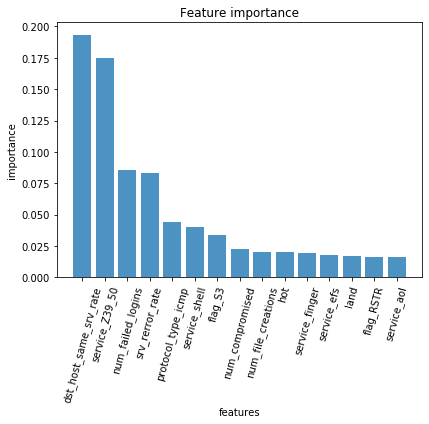
\includegraphics[width=0.7\linewidth]{img/extratree.png}
    \caption{Top 15 feature by importance as per ExtraTree Classifier ranking}
    \label{fig:classtree}
\end{figure}

%-------
\subsection{Univariate Selection}

Univariate feature selection is another method provided by the \texttt{scikit-learn} collection: it examines each feature individually to determine the strength of the relationship of the feature with the response variable \cite{univ}.

Figure~\ref{fig:classuniv} shows the best 15 features found with Univariate Selection. 

\begin{figure}[h]
    \centering
    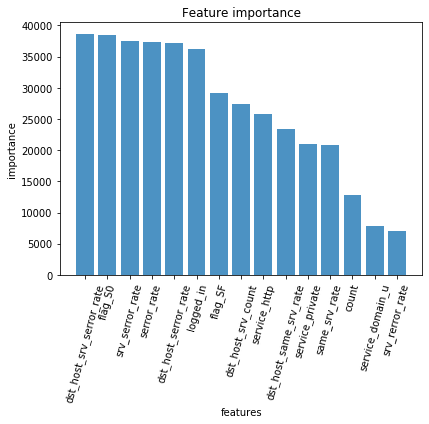
\includegraphics[width=0.7\linewidth]{img/univ.png}
    \caption{Top 15 feature by importance as per Univariate Selection ranking}
    \label{fig:classuniv}
\end{figure}

\FloatBarrier